	\documentclass[10pt,oneside]{CBFT_book}
	% Algunos paquetes
	\usepackage{amssymb}
	\usepackage{amsmath}
	\usepackage{graphicx}
	\usepackage{libertine}
	\usepackage[bold-style=TeX]{unicode-math}
	\usepackage{lipsum}

	\usepackage{natbib}
	\setcitestyle{square}

	\usepackage{polyglossia}
	\setdefaultlanguage{spanish}


	\usepackage{CBFT.estilo} % Cargo la hoja de estilo

	% Tipografías
	% \setromanfont[Mapping=tex-text]{Linux Libertine O}
	% \setsansfont[Mapping=tex-text]{DejaVu Sans}
	% \setmonofont[Mapping=tex-text]{DejaVu Sans Mono}

	%===================================================================
	%	DOCUMENTO PROPIAMENTE DICHO
	%===================================================================

\begin{document}

% =================================================================================================
\chapter{Campos de cargas en movimiento}
% =================================================================================================

% =================================================================================================
\section{Potenciales retardados}
% =================================================================================================

Usando el gauge de Lorentz y las ecuaciones de Maxwell se llega a
\[
	\lapm{\vb{A}} - \frac{1}{c^2} \dpar[2]{\vb{A}}{t} = -\frac{4\pi}{c} \vb{J}
\]
\[
	\lapm{\phi} - \frac{1}{c^2} \dpar[2]{\phi}{t} = - 4 \pi \phi
\]
con forma general 
\be
	\lapm{\psi} - \frac{1}{c^2} \dpar[2]{\psi}{t} = - 4 \pi f(\vb{x},t)
	\label{onda_general}
\ee
siendo $f$ la que da la distribución de fuentes.

Resolveremos \eqref{onda_general} con una función de Green. Hacemos Fourier respecto a la frecuencia, de
manera que podamos remover el tiempo (además luego nos interesarán fuentes armónicas y por sobre todo
cualquier perturbación puede descomponerse en Fourier).

Suponemos que podemos escribir
\[
	\psi(\vb{x},t) = \frac{1}{2\pi}\int_{-\infty}^{+\infty} \psi(\vb{x},\omega) \euler^{-i\omega t} 
	d\omega
\]
\[
	f(\vb{x},t) = \frac{1}{2\pi}\int_{-\infty}^{+\infty} f(\vb{x},\omega) \euler^{-i\omega t} d\omega
\]
siendo sus inversas
\[
	\psi(\vb{x},\omega) = \int_{-\infty}^{+\infty} \psi(\vb{x}, t) \euler^{i\omega t} dt
\]
\[
	f(\vb{x},\omega) = \int_{-\infty}^{+\infty} f(\vb{x},t) \euler^{i\omega t} dt
\]
luego la ecuación resulta 
\[
	\int_{-\infty}^{+\infty} \lapm{\psi}(\vb{x},\omega) \euler^{ -i\omega t} d\omega +
	\int_{-\infty}^{+\infty} \frac{\omega^2}{c^2}\psi(\vb{x},\omega) \euler^{ -i\omega t} d\omega = 
		- 4 \pi \int_{-\infty}^{+\infty} f(\vb{x},\omega) \euler^{ -i\omega t} d\omega
\]
de manera que se satisface la ecuación de Helmholtz inhomogénea,
\[
	(\nabla^2 + k^2)\psi(\vb{x},\omega) = - 4\pi f(\vb{x},\omega),
\]
para cada valor de frecuencia $\omega$.

Una función de Green satisfacerá 
\[
	(\nabla^2 + k^2) G(\vb{x},\vb{x}') = - 4\pi \delta(\vb{x}-\vb{x}'),
\]
donde $\vb{x}-\vb{x}' = \vb{R}$ y la función de Green será simétricamente esférica pues pedimos la
no existencia de contornos, entonces llamando a aquella $G_k(R)$ se tiene 
\[
	\frac{1}{R}\dtot[2]{}{R}(RG_k) + k^2 G_k = - 4 \pi \delta (\vb{R})
\]
donde hemos usado el laplaciano en esféricas. Debemos distinguir dos casos, si $R=0$ entonces la
anterior resulta 
\[
	\lim_{kR \to 0} G_k(R) = \frac{1}{R}
\]
mientras que de ser cierto $R\neq 0$ en cambio
\[
	\dtot[2]{}{R}(RG_k) + k^2 (RG_k) = 0
\]
y entonces se propone como solución general 
\[
	G_k(R) = \frac{ A }{ R } \euler^{ i k R } + \frac{ B }{ R } \euler^{ -i k R }
\]
donde $A, B$ dependerán de las condiciones de contorno y siendo que el primer término del RHS representa
una onda divergente esférica y el segundo una onda convergente esférica.

Se puede interpretar $G_k$ como el potencial de una carga unitaria que aparece en $\vb{x}=\vb{x}'$ en el
instante $t=t'$ y luego desaparece (mmm, qué misterio!).

Ahora necesitamos meter la dependencia temporal,
\[
	\left(\nabla^2_x - \frac{1}{c^2}\dpar[2]{}{t} \right) G^{\pm}(\vb{x},\vb{x}',t,t') = 
	- 4 \pi \delta(\vb{x}-\vb{x}') \delta(t-t')
\]
\[
	- 4 \pi f(\vb{x},\omega) = -4 \pi \int_{-\infty}^{+\infty} f(\vb{x},t) \euler^{i\omega t} dt =
		-4 \pi \int_{-\infty}^{+\infty} \delta(\vb{x}-\vb{x}') \delta(t-t') \euler^{i\omega t} dt
\]
\[
	- 4 \pi f(\vb{x},\omega) = -4 \pi \delta(\vb{x}-\vb{x}') \euler^{i\omega t'} 
\]
de modo que tenemos 
\[
	f(\vb{x},\omega) = \delta(\vb{x}-\vb{x}') \euler^{i\omega t'} ,
\]
usando lo cual se llega a
\[
	G^{\pm}(R,\tau) = \frac{1}{2\pi} \int_{-\infty}^{+\infty} G_k(R) \euler^{-\omega t} d\omega
\]
donde $\tau$ es el tiempo relativo entre los tiempos de observación y fuente ($t'$ ) y $R$ es la distancia 
relativa entre observación y fuente.

En un medio no dispersivo es 
\[
	G^{\pm}(R,\tau) = \frac{1}{R} \delta( \tau \mp \frac{R}{c})
\]
y así llegamos a
\[
	G^+(\vb{x},\vb{x}',t,t') = \frac{1}{|\vb{x} - \vb{x}'|} \delta( t-t' - \frac{1}{c}(\vb{x} - 
	\vb{x}')) = \frac{ \delta(t' - [t-(1/c)|\vb{x} - \vb{x}'|]) }{|\vb{x} - \vb{x}'|} ,
\]
la función de Green retardada
\[
	G^-(\vb{x},\vb{x}',t,t') = \frac{1}{|\vb{x} - \vb{x}'|} \delta( t-t' + \frac{1}{c}(\vb{x} - 
	\vb{x}')) = \frac{ \delta(t' - [t + (1/c)|\vb{x} - \vb{x}'|]) }{|\vb{x} - \vb{x}'|},
\]
la función de Green avanzada.

$G^+$ exhibe el comportamiento causal del efecto observado en \vb{x} a $t$ causado por la acción de la
fuente en el tiempo $(t-R/c)$ donde $R/c$ es la diferencia de tiempo de la señal en propagarse.
Al valor 
\[
	t' = t - \frac{R}{c}
\]
se lo llama el tiempo retardado. Es un poco más práctica la nomenclatura
\[
	G^+(R,t,t') = \frac{ \delta(t' - [ t - (R/c) ]) }{ R } 
	\qquad 
	G^-(R,t,t') = \frac{ \delta(t' - [ t + (R/c) ]) }{ R } ,
\]

Entonces una solución particular de (1) (¿uno qué?) es 
\[
	\psi^\pm (\vb{x},t) = \int \int G^{\pm}(\vb{x},\vb{x}',t,t') f(\vb{x}',t') d^3x' dt' 
\]
y dos soluciones son 
\[
	\psi_{in}(\vb{x},t) + \int\int G^+ f dv' dt \qquad \qquad \psi_{s}(\vb{x},t) + \int\int G^- f dv' dt
\]
con $f(\vb{x}',t')$ una fuente que es diferente de cero solo en un intervalo $\sim t'$. Entonces $\psi_{in}$ 
satisface (1) homogénea en $t \to -\infty$. $\psi_{s}$ es la onda en $t \to +\infty$ solución homogénea.
La situación más común es el caso de $\psi_{in}$ con $\psi_{in}=0$ entonces 
\[
	\psi (\vb{x},t) = \int_{-\infty}^{+\infty} \int_v' \frac{\delta(t'-[t -(R/c) ]) }{ R } 
			f(\vb{x}',t') dv' dt',
\]
e integrando con la delta
\[
	\psi (\vb{x},t) = \int_v' \frac{ f( \vb{x}', t -(R/c) ) }{ R } dv',
\]
que es una fuente en una cierta región que se enciende un instante e irradia.

\subsection{Fuente armónica}

Sea una fuente armónica en el tiempo 
\[
	\vb{J}(\vb{x}', t') = \vb{J}(\vb{x}') \euler^{-i\omega t'}
\]
entonces el potencial vector es 
\[
	\vb{A}(\vb{x}, t) = \left. \frac{4\pi}{c} \int_v' \frac{\vb{J}(\vb{x}')}{|\vb{x} - \vb{x}'|} 
	\euler^{-i\omega t'} \right|_{t_{ret}} dv' = \left. \frac{4\pi}{c} \int_v' 
	\frac{\vb{J}(\vb{x}')}{|\vb{x} - \vb{x}'|} \euler^{-i \omega t} \euler^{i \omega R/c } 
	\right|_{t_{ret}} dv'
\]
\[
	\vb{A}(\vb{x}, t) = \frac{4\pi}{c} \euler^{-i \omega t} \int_v \frac{\vb{J}(\vb{x})}{ R }
		\euler^{i \omega R/c } dv
\]
se puede ver como 
\[
	\vb{A}(\vb{x}) \euler^{-i \omega t} = \frac{4\pi}{c} \int_v' \frac{\vb{J}(\vb{x}')}{|\vb{x}-\vb{x}'|}
		\euler^{i k |\vb{x}-\vb{x}'| } dv' \euler^{-i \omega t}
\]

Si la fuente oscila armónicamente con frecuencia $\omega$ entonces los campos tendrán la misma frecuencia 
$\omega$.
\[
	\vb{A}(\vb{x}) = \frac{1}{c} \int_v' \frac{\vb{J}(\vb{x}')}{|\vb{x}-\vb{x}'|}
		\euler^{i \omega/c |\vb{x}-\vb{x}'| } dv'
\]
y 
\[
	\vb{A}(\vb{x},t) = \vb{A}(\vb{x}) \euler^{-i \omega t} \quad \text{si} \quad
		\vb{J}(\vb{x}',t') = \vb{J}(\vb{x}') \euler^{-i \omega t'}
\]
La aproximación consiste en desarrollar 
\[
	\frac{\euler^{i k |\vb{x}-\vb{x}'| }}{|\vb{x}-\vb{x}'|}
\]
y ver condiciones asintóticas. Cuando $\ell = 0$ (el primer término de la sumatoria en $\ell$) y
$ kx' \ll 1$ tenemos una antena ineficiente. La longitud de onda $\lambda$ de la radiación es mucho mayor al 
tamaño del emisor, $ 2\pi x' \ll \lambda$ (longitud de onda larga).
En cambio tenemos $ 2\pi x \gg \lambda$ que es la condición de campo lejano (siempre la usaremos).

Por lo tanto,
\[
	\vb{A}(\vb{x})^{(0)} = - i k \vb{p} \frac{\euler^{ikx}}{x}
\]
es una onda esférica saliente. Es el potencial vector \vb{A} de un dipolo magnético oscilante armónicamente.
Recordemos que falta siempre {\it pegarle} un factor $\exp(i\omega t)$. Usando $\vb{E} 0 i/k \rotorm{B}, 
\vb{B} = \rotorm{A}$ tenemos 
\be
	\vb{B}(\vb{x})^{(0)} = k^2 (\hat{r}\times\vb{p})\frac{\euler^{ikx}}{x}\left(1 -\frac{1}{ikx}\right)
	\label{B_rad}
\ee
siendo $\hat{r}$ la dirección de propagación y $x\equiv|\vb{x}|$ que puede ser $|r\hat{r}|$ en esféricas.
El que contribuye a la radiación es el primer término de \eqref{B_rad} (campo lejano) mientras que el segundo
se va a cero rápidamente.

Cerca de la antena es 
\[
	\vb{B}(\vb{x})^{(0)} = i k (\hat{r}\times\vb{p})\frac{1}{r^2}, 
\]
pues $kx\ll 1$ y entonces $\exp(ikx) \sim 1$ (campo cercano) de manera que si $\lambda \to \infty$ entonces
$\vb{B}^{(0)} \sim 0$. El campo \vb{E} cerca de la antena es
\[
	\vb{E} = \frac{i}{k}\rotorm{B} \qquad \rightarrow \quad 
	\vb{E}^{(0)} = \frac{3\hat{r}(\hat{r}\cdot\vb{p}) - \vb{p}}{r^3}
\]
que es el campo de un dipolo eléctrico. $\vb{E},\vb{B}$ son transversales a $\hat{r}$ y tienen la misma 
longitud (en unidades CGS).
La potencia media (en un número entero de períodos) será 
\[
	\langle dP \rangle = \langle\vb{S}\rangle\cdot d\vb{S} = \langle \vb{S}\rangle\cdot\hat{n}r^2 d\Omega
\]
y entonces
\[
	\langle\frac{dP}{d\Omega}\rangle = \langle\vb{S}\rangle\cdot\hat{n}r^2 
\]
\[
	\langle\frac{dP}{d\Omega}\rangle = \frac{c}{8\pi} k^4 p^2 \sin(\theta)^2 
\]
y este cálculo podemos ver de dónde sale 
\[
	\langle\vb{S}\rangle = \frac{c}{2 4 \pi} \re\{ \vb{E}\times\vb{B}^* \} =
		\frac{c}{8\pi} \re\{ ( \vb{B}^0 \times \hat{r} )\times k^2(\hat{r} \times \vb{p})/r \}
\]
\[
	\langle\vb{S}\rangle =
	\frac{c}{8\pi} \re\{(-p k^2/r \sin(\theta) \hat{\theta})\times(-p k^2/r\sin(\theta)\hat{\phi} \}
	= \frac{c}{8\pi} p^2 k^4 \sin(\theta)^2 \hat{r}\cdot\hat{r}
\]
\notamargen{Tenemos un cálculo auxiliar de esta cuenta pero no sé si suma meterlo acá.}

Luego, la potencia irradiada es máxima en $\theta=\pi/2$ (ver figura)

\begin{figure}[htb]
	\begin{center}
	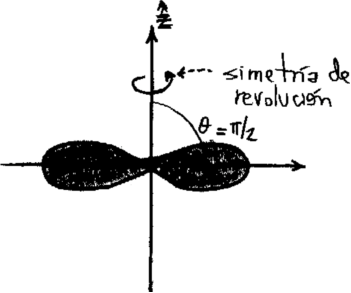
\includegraphics[width=0.4\textwidth]{images/fig_ft1_pot_irrad.pdf}	 
	\end{center}
	\caption{}
\end{figure} 

Entonces, 

\begin{figure}[htb]
	\begin{center}
	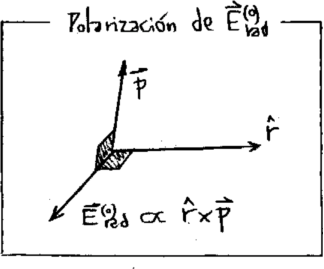
\includegraphics[width=0.4\textwidth]{images/fig_ft1_pot_irrad2.pdf}	 
	\end{center}
	\caption{}
\end{figure} 

\begin{figure}[htb]
	\begin{center}
	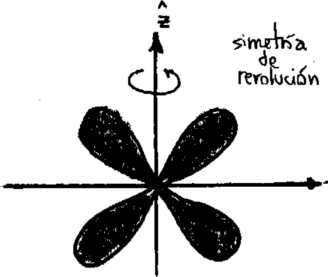
\includegraphics[width=0.4\textwidth]{images/fig_ft1_pot_irrad3.pdf}	 
	\end{center}
	\caption{}
\end{figure} 

% =================================================================================================
\section{Ejemplo de antena}
% =================================================================================================

\begin{figure}[htb]
	\begin{center}
	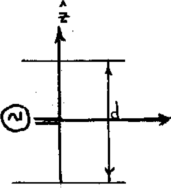
\includegraphics[width=0.4\textwidth]{images/fig_ft1_antena.pdf}	 
	\end{center}
	\caption{}
\end{figure} 

\begin{figure}[htb]
	\begin{center}
	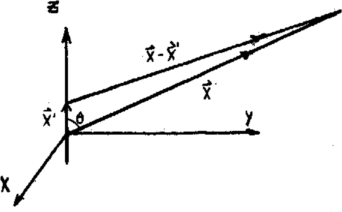
\includegraphics[width=0.4\textwidth]{images/fig_ft1_antena2.pdf}	 
	\end{center}
	\caption{}
\end{figure} 


\begin{figure}[htb]
	\begin{center}
	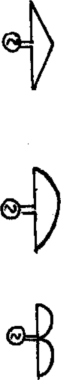
\includegraphics[width=0.4\textwidth]{images/fig_ft1_antena3.pdf}	 
	\end{center}
	\caption{}
\end{figure} 

% =================================================================================================
\section{Campos de una partícula cargada en movimiento}
% =================================================================================================

\begin{figure}[htb]
	\begin{center}
	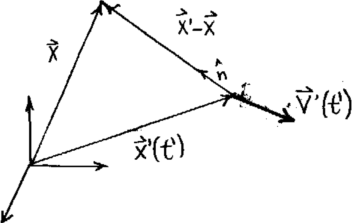
\includegraphics[width=0.4\textwidth]{images/fig_ft1_campo_part_car.pdf}	 
	\end{center}
	\caption{}
\end{figure} 

\begin{figure}[htb]
	\begin{center}
	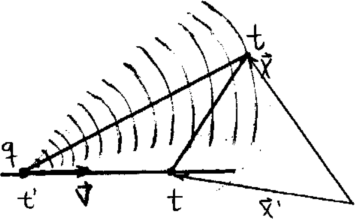
\includegraphics[width=0.4\textwidth]{images/fig_ft1_campo_part_car2.pdf}	 
	\end{center}
	\caption{}
\end{figure} 

% =================================================================================================
\section{Campo de una carga en movimiento}
% =================================================================================================

\begin{figure}[htb]
	\begin{center}
	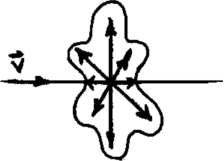
\includegraphics[width=0.4\textwidth]{images/fig_ft1_campo_carga_mov.pdf}	 
	\end{center}
	\caption{}
\end{figure} 

\begin{figure}[htb]
	\begin{center}
	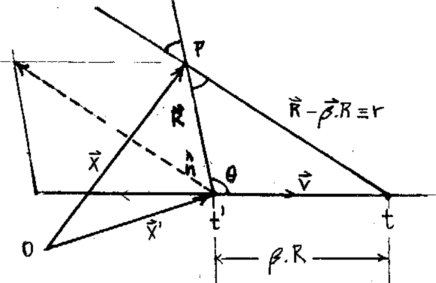
\includegraphics[width=0.4\textwidth]{images/fig_ft1_campo_carga_mov2.pdf}	 
	\end{center}
	\caption{}
\end{figure} 

% =================================================================================================
\section{Cálculo de potencia irradiada}
% =================================================================================================

\begin{figure}[htb]
	\begin{center}
	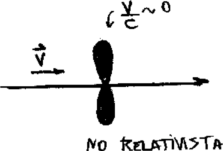
\includegraphics[width=0.4\textwidth]{images/fig_ft1_frenado2.pdf}	 
	\end{center}
	\caption{}
\end{figure} 

\begin{figure}[htb]
	\begin{center}
	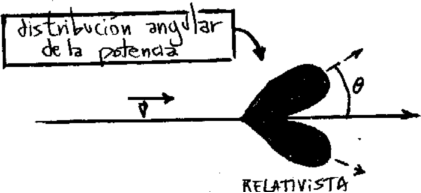
\includegraphics[width=0.4\textwidth]{images/fig_ft1_frenado3.pdf}	 
	\end{center}
	\caption{}
\end{figure} 

% =================================================================================================
\section{Frenado magnético}
% =================================================================================================

\begin{figure}[htb]
	\begin{center}
	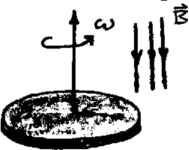
\includegraphics[width=0.4\textwidth]{images/fig_ft1_frenado.pdf}	 
	\end{center}
	\caption{}
\end{figure} 

% =================================================================================================
\subsection{Esponja electromagnética}
% =================================================================================================

\begin{figure}[htb]
	\begin{center}
	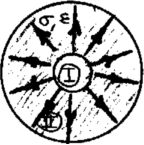
\includegraphics[width=0.4\textwidth]{images/fig_ft1_esponja.pdf}	 
	\end{center}
	\caption{}
\end{figure} 

% \bibliographystyle{CBFT-apa-good}	% (uses file "apa-good.bst")
% \bibliography{CBFT.Referencias} % La base de datos bibliográfica

\end{document}
